\section{Norme IEEE 754}
%TODO brève expliquation de comment fonctionnent les nombres flotants

\section{Différences entre calculs sur CPU et GPU}
\subsection{Observations}
Cuda supporte la norme IEEE 754 pour les calculs avec nombre flottants \cite{Cuda_IEEE754}. Toutefois, la première implémentation Cuda de la \acs{LBM} a montré des différences sur certains calculs réalisés par les codes \ac{CPU}.

\subsection{Mesures}
Pour mesurer cette différence, un code \ac{LBM} $2D$ \ac{CPU} et un code \ac{GPU} ont été implémenté et leurs résultats comparés. La figure \ref{fig:lbm_float_deltas} illustre la différence moyenne entre les valeurs calculées sur \ac{CPU} et \ac{GPU} pour l'ensemble des populations $f_{in}$ de chaque itération.

\begin{figure}[h]
	\centering
	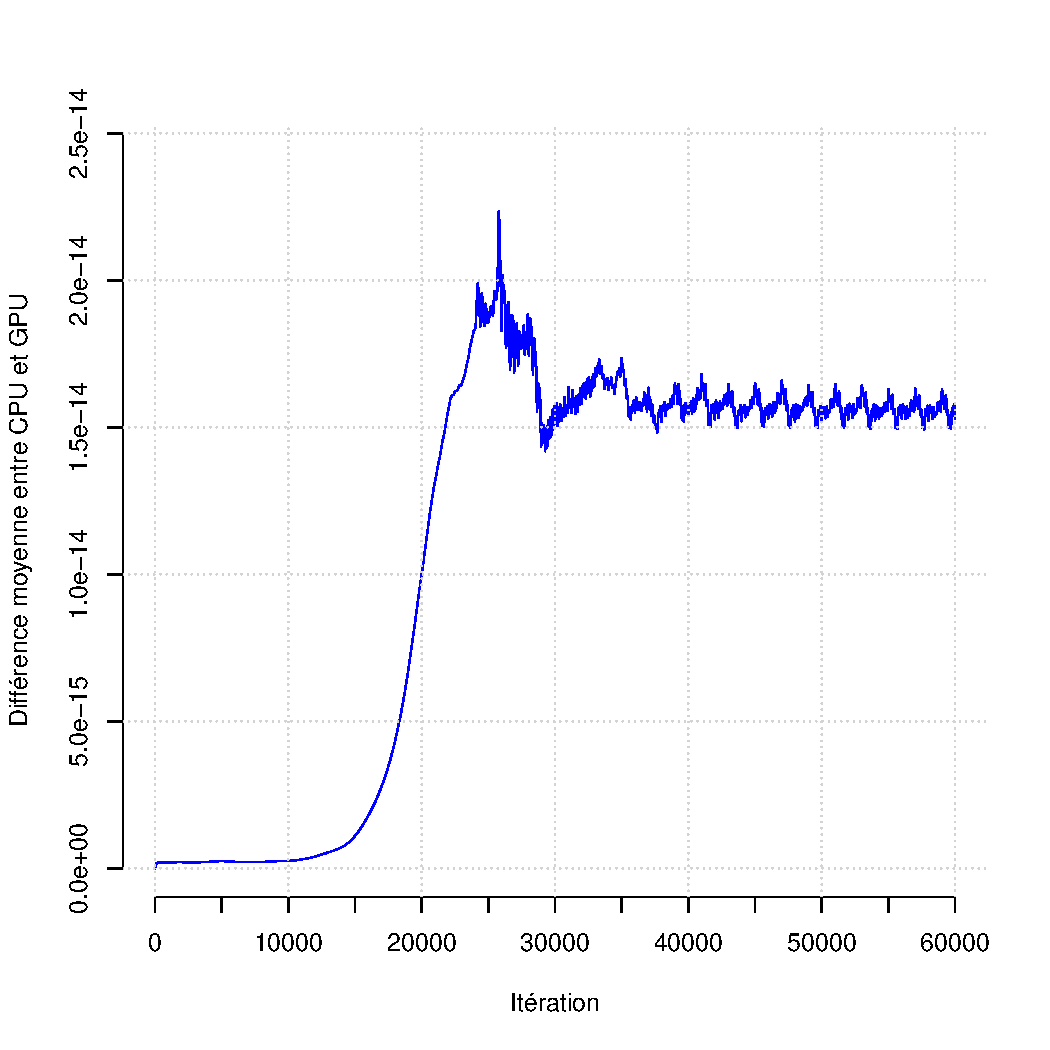
\includegraphics[scale=0.75, fbox]{../data/lbm_cpu_vs_gpu/deltas/Rplots.pdf}
	\caption{Différences moyennes (par itération) entre les calculs sur \acs{CPU} et \acs{GPU}}
	\label{fig:lbm_float_deltas}
\end{figure}

L'écart entre les résultats observés sur \ac{CPU} et \ac{GPU} suit les étapes de la simulation réalisée (fluide autour d'un cylindre) illustrée par les figures \ref{fig:lbm_5000_to_43000}:
\begin{itemize}
\item entre 0 et environ 12000 itérations, la queue se forme derrière le cylindre et la l'écart moyen reste faible et stable (quinze zéros après la virgule);
\item entre 15000 et 20000 itérations, la queue commence à osciller et l'écart augmente brutalement (treize zéros après la virgule);
\item à la 25792$^{\textrm{ième}}$ itération, l'oscillation commence à se stabiliser et l'écart atteint son maximum (toujours treize chiffres après la virgule);
\item dès environ 36000 itérations, l'oscillation est stabilisée (comme le montre les figure \ref{fig:lbm_39000} et \ref{fig:lbm_43000}, même motif réapparaît toute les 4000 itérations environ) et les écarts avec.
\end{itemize}

La différence entre certains résultats sur \ac{CPU} et \ac{GPU} est le fruit d'une optimisation du compilateur Cuda. 

\begin{figure}[h]
	\centering
	\subfigure[5000 itérations]{%
		\centering
		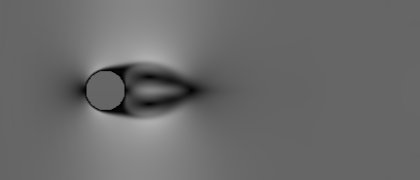
\includegraphics[scale=0.5]{../data/lbm_images/cpu_lbm_5000.png}
		\label{fig:lbm_5000}
	}
	\subfigure[10000 itérations]{%
		\centering
		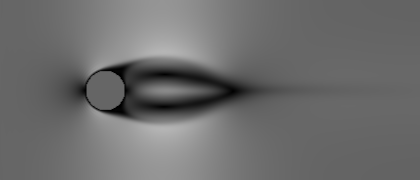
\includegraphics[scale=0.5]{../data/lbm_images/cpu_lbm_10000.png}
		\label{fig:lbm_10000}
	}
	\subfigure[15000 itérations]{%
		\centering
		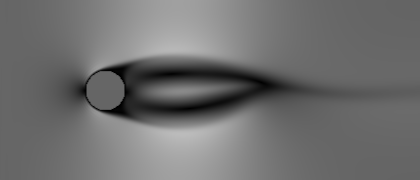
\includegraphics[scale=0.5]{../data/lbm_images/cpu_lbm_15000.png}
		\label{fig:lbm_15000}
	}
	\subfigure[20000 itérations]{%
		\centering
		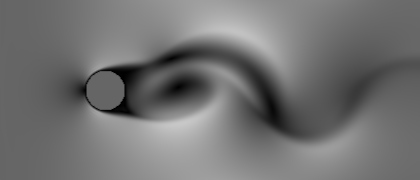
\includegraphics[scale=0.5]{../data/lbm_images/cpu_lbm_20000.png}
		\label{fig:lbm_20000}
	}
	\subfigure[25792 itérations]{%
		\centering
		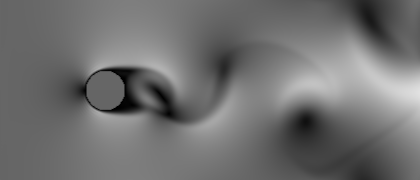
\includegraphics[scale=0.5]{../data/lbm_images/cpu_lbm_25792.png}
		\label{fig:lbm_25792}
	}
	\subfigure[39000 itérations]{%
		\centering
		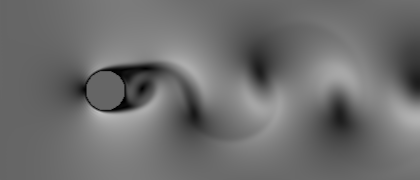
\includegraphics[scale=0.5]{../data/lbm_images/cpu_lbm_39000.png}
		\label{fig:lbm_39000}
	}
	\subfigure[40000 itérations]{%
		\centering
		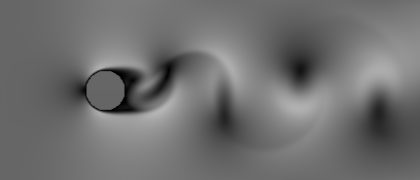
\includegraphics[scale=0.5]{../data/lbm_images/cpu_lbm_40000.png}
		\label{fig:lbm_40000}
	}
	\subfigure[41000 itérations]{%
		\centering
		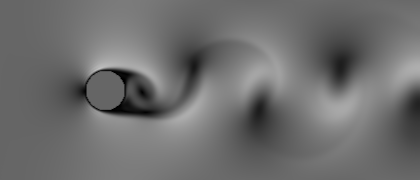
\includegraphics[scale=0.5]{../data/lbm_images/cpu_lbm_41000.png}
		\label{fig:lbm_41000}
	}
	\subfigure[42000 itérations]{%
		\centering
		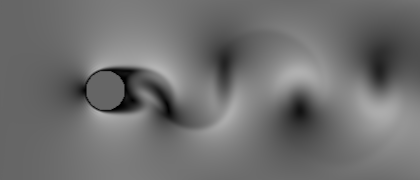
\includegraphics[scale=0.5]{../data/lbm_images/cpu_lbm_42000.png}
		\label{fig:lbm_42000}
	}
	\subfigure[43000 itérations]{%
		\centering
		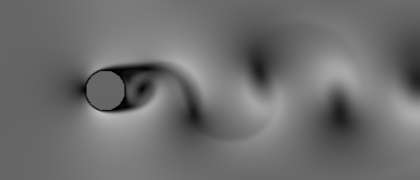
\includegraphics[scale=0.5]{../data/lbm_images/cpu_lbm_43000.png}
		\label{fig:lbm_43000}
	}
	\caption{Simulation \ac{LBM} d'un fluide autour d'un cylindre}
	\label{fig:lbm_5000_to_43000}
\end{figure}

\subsection{Fonctions intrinsèques}
Sur \ac{CPU}, lorsqu'une opération du type $r = x \times y+z$ est rencontrée, le processeur calcul d'abord $r_{xy} = x \times y$ puis $r = r_{xy} + z$. Deux opérations sont donc réalisées, ce qui implique deux potentiels arrondis dans le cas des nombres flottants. Sur \ac{GPU}, le compilateur optimise ce type de calculs \cite{Cuda_IEEE754_Ctrl_FMA} avec la fonction \ac{FMA} qui réalise $x \times y+z$ en une seule opération. Le calcul est ainsi plus rapide et précis (puisqu'un seul arrondi est effectué).

Comme le souligne la documentation de Cuda, cette optimisation n'est pas forcément souhaitable dans certaines circonstances et peut être évitée avec l'utilisation de fonctions intrinsèques \cite{Cuda_IEEE754_Ctrl_FMA, Cuda_INTRINSIC_DOUBLE}.

Cette précaution force le \ac{GPU} à effectuer les multiplications et additions indépendamment et permet de s’assurer que les calculs réalisés sur \ac{CPU} et \ac{GPU} produisent les mêmes résultats.
